\documentclass[letterpaper]{article}
\usepackage[submission]{aaai2027}
\usepackage{graphicx}
\usepackage{booktabs}
\usepackage{amsmath}
\usepackage{amssymb}
\usepackage{microtype}
\usepackage[hyphens]{url}
\usepackage{natbib}
\usepackage{caption}
\frenchspacing
\setlength{\pdfpagewidth}{8.5in}
\setlength{\pdfpageheight}{11in}
\pdfinfo{/TemplateVersion (2027.1)}
\setcounter{secnumdepth}{2}

\title{STAFF: Stress-Testing Adaptation for Full-Page Optical Music Recognition}
\author{Anonymous Submission}
\affiliations{}

\begin{document}
\maketitle

\begin{abstract}
Optical music recognition (OMR) systems are commonly evaluated within the same rendered or scanned collection used for training, although practical deployment crosses engraving engines, repertoires, layouts, vocabularies, and capture conditions. We present STAFF, a controlled study of cross-domain adaptation for pianoform and full-page OMR. STAFF separates two complementary paths: a modular, staff-aware detector--segmenter--graph pipeline that exposes intermediate errors, and adaptation of released image-to-sequence models under fixed target-label budgets. Across OLiMPiC, GrandStaff-LMX, FP-GrandStaff, and scanned Polish scores, we retain the official or dataset-compatible tokenization and metric implementation and report zero-, 100-, and 1000-page settings where available. A released OLiMPiC sequence model obtains 53.19\% Symbol Error Rate (SER) when transferred directly to the 200-page GrandStaff-LMX test split; adaptation with 100 and 1000 target pages reduces SER to 38.18\% and 14.01\%, respectively. Reverse transfer remains harder: adapting a GrandStaff model with 100 OLiMPiC pages reduces SER from 56.49\% to 51.79\%. The modular path runs without target-domain sequence training but remains semantically weak, localizing the dominant bottleneck in pitch, duration, voice, and structural decoding rather than page parsing alone. These results support a simple conclusion: OMR transfer should be reported as a label-budget curve with explicit ownership, protocol, and failure categories, rather than as a single in-domain score.
\end{abstract}

\section{Introduction}
Optical music recognition converts score images into machine-readable notation. Unlike ordinary character recognition, the meaning of a mark depends jointly on its class, staff-relative position, attachment relations, voice, and reading order \cite{calvozaragoza2021understanding,rebelo2012optical}. Modern systems increasingly treat OMR as image-to-sequence prediction, using Transformer decoders to emit compact musical encodings \cite{vaswani2017attention,riosvila2024smt,li2023tromr}. This formulation has enabled recognition beyond monophonic incipits and toward piano systems or complete pages \cite{riosvila2023grandstaff,riosvila2026fullpage}. Yet the apparent progress hides a deployment problem: a model trained on one renderer, score collection, vocabulary, or page layout can fail sharply on another.

The shift is visible before any model is run. Synthetic piano pages have clean backgrounds, regular spacing, and constrained engraving, whereas scanned historical scores contain uneven contrast, page texture, warped systems, typography changes, and more varied annotations. Figure~\ref{fig:domain} contrasts representative pages in the local evaluation collections. The output space shifts as well: Humdrum-based encodings, Linearized MusicXML (LMX), tuplets, voices, and staff markers differ in vocabulary and structural assumptions. General transfer-learning results predict that higher model layers become increasingly task-specific \cite{pan2010transfer,yosinski2014transferable}; for OMR, the decoder and notation vocabulary are precisely the most domain-specific components.

\begin{figure}[t]
  \centering
  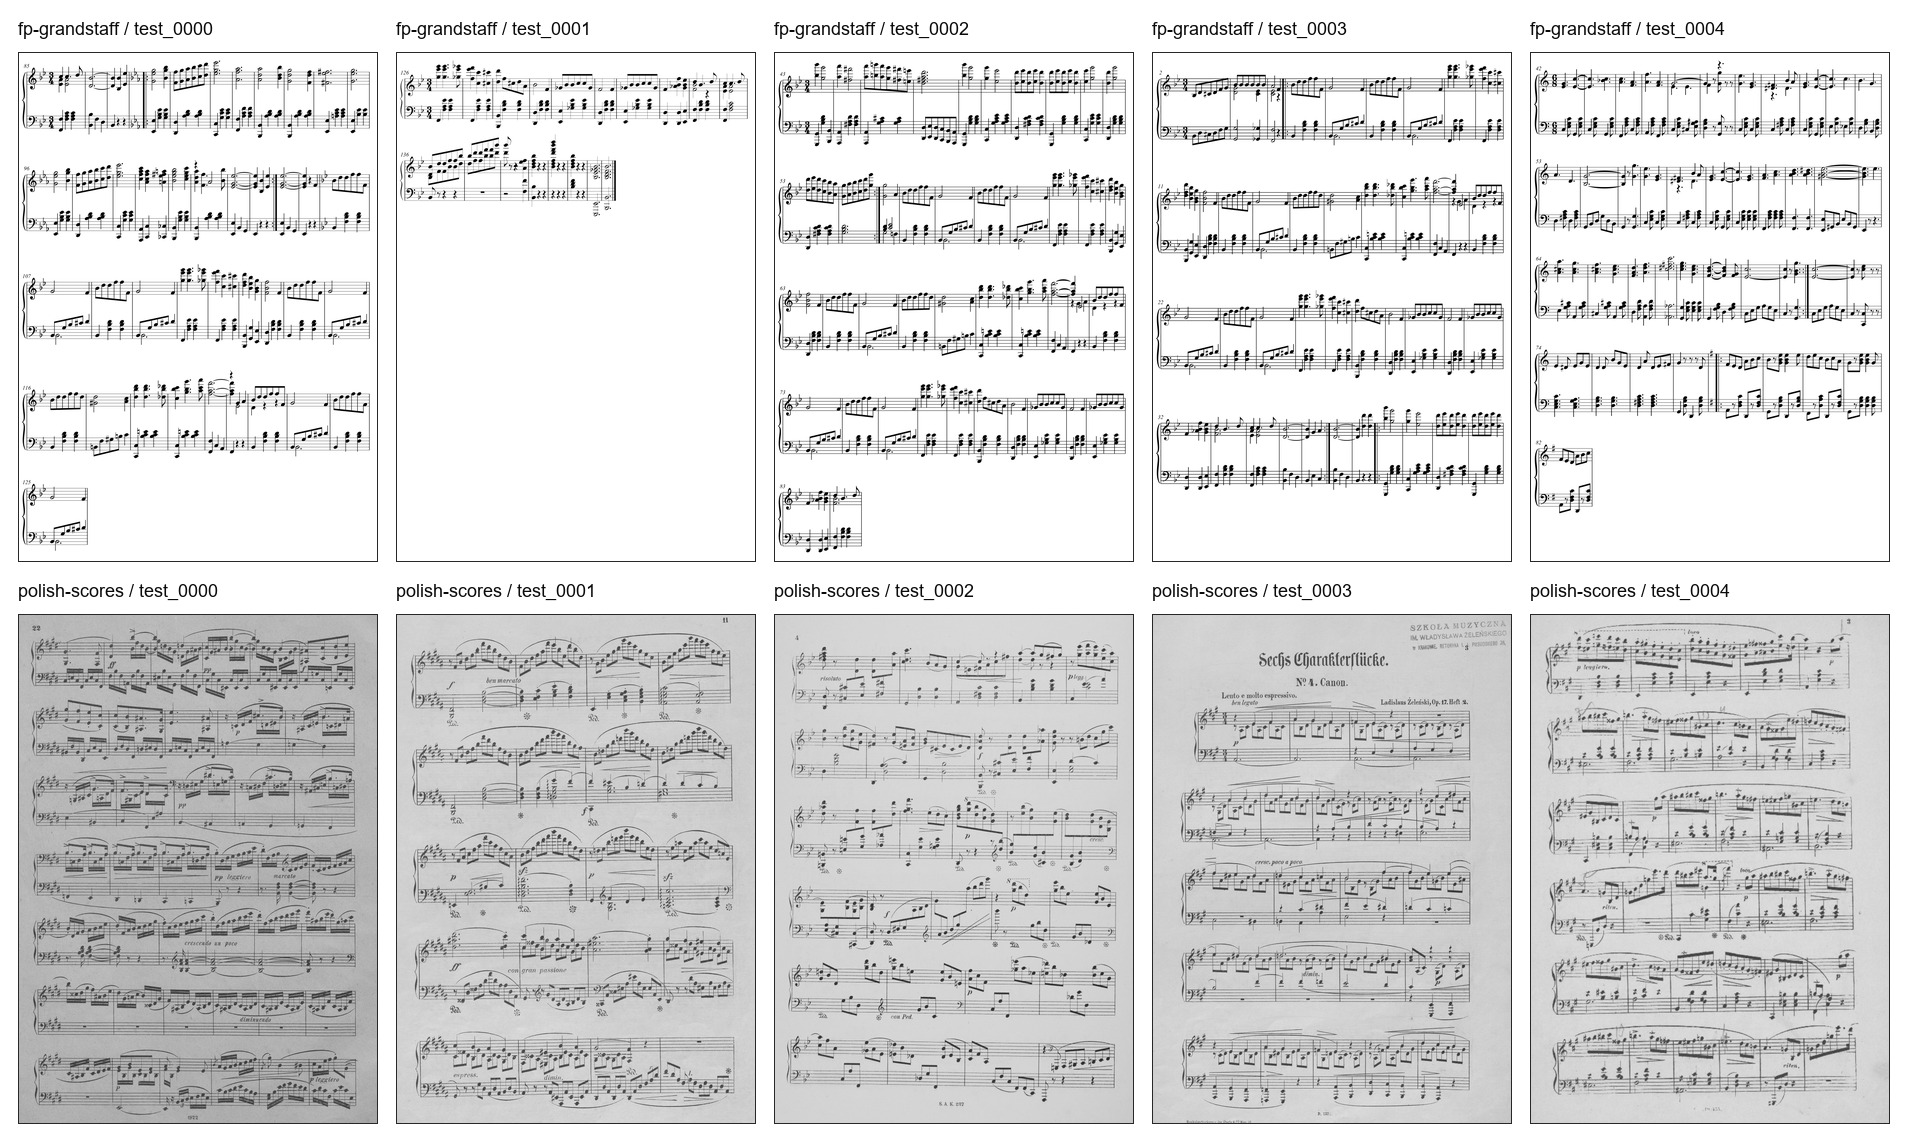
\includegraphics[width=\linewidth]{domain_shift.jpg}
  \caption{Representative synthetic FP-GrandStaff pages (top) and scanned Polish pages (bottom). The target shift changes appearance, page density, typography, and annotation vocabulary simultaneously.}
  \label{fig:domain}
\end{figure}

This paper introduces STAFF, short for \emph{Stress-Testing Adaptation for Full-Page OMR}. STAFF is not a new claim that one architecture solves all domains. It is an evidence protocol and a paired implementation that makes transfer behavior inspectable. One path uses a modular StaffOMR-SAM pipeline: staff geometry establishes a normalized coordinate frame; DEIM-D-FINE detects symbols; SAM2 refines boxes into masks; class-conditioned geometry produces polygons, skeletons, relations, and draft MusicXML/LMX. The other path adapts released image-to-sequence weights with controlled target-label budgets. Both paths are evaluated with fixed splits and the metric implementation associated with the output encoding.

Our contributions are threefold:
\begin{itemize}
  \item We provide a controlled bidirectional transfer matrix across OLiMPiC, GrandStaff-LMX, FP-GrandStaff, and scanned Polish scores, separating zero-shot, 100-page, and 1000-page regimes and distinguishing released architectures from our adaptation experiments.
  \item We show that target labels produce a strongly nonlinear transfer curve: on GrandStaff-LMX test200, 1000-page adaptation reduces official LMX SER from 53.19\% to 14.01\%, while 100 pages reach 38.18\% and reverse transfer remains much weaker.
  \item We pair the sequence results with an interpretable detector--mask--relation pipeline and an error taxonomy, showing that robust symbol localization alone does not resolve missing pitch, duration, voice, and MusicXML structure.
\end{itemize}

\section{Related Work}
\subsection{Datasets and Modular OMR}
OMR research has historically decomposed a page into staff detection, symbol recognition, and notation reconstruction \cite{calvozaragoza2021understanding,rebelo2012optical}. Dataset design reflects this decomposition. MUSCIMA++ provides handwritten symbols and explicit pairwise relations, enabling notation-graph experiments \cite{hajic2017muscima}. DeepScores and DeepScoresV2 provide dense synthetic annotations for tiny printed objects, instance segmentation, and detection \cite{tuggener2018deepscores,tuggener2020deepscoresv2}. Camera-PrIMuS supports end-to-end recognition under realistic image degradation but is primarily monophonic \cite{calvozaragoza2018primus}. RealScores and recent instance-segmentation studies further emphasize that real-world score images differ materially from synthetic renders \cite{shatri2023realworld,shatri2024segmentation}.

Object-centric OMR benefits from detectors that preserve small, dense instances. DETR introduced set prediction with bipartite matching \cite{carion2020detr}; RT-DETRv2, D-FINE, and DEIM improve multiscale sampling, localization, and convergence \cite{lv2024rtdetrv2,peng2025dfine,huang2025deim}. Promptable segmentation offers a complementary route from boxes to boundaries. SAM established zero-shot promptable segmentation \cite{kirillov2023segment}, while SAM2 extended the design and improved image efficiency \cite{ravi2025sam2}. STAFF uses these models as reusable components, not as evidence that natural-image priors alone understand notation semantics. DINOv2 features support retrieval and crop-level auxiliary classification \cite{oquab2023dinov2}, but all final claims are based on end-output metrics rather than embedding similarity.

\subsection{End-to-End Pianoform Recognition}
GrandStaff introduced a large pianoform corpus and a sequence-recognition formulation over kern-like encodings \cite{riosvila2023grandstaff}. Sheet Music Transformer extended image-to-sequence OMR beyond monophonic transcription \cite{riosvila2024smt}, and full-page variants combined convolutional encoders, autoregressive decoders, synthetic curriculum learning, and target-domain fine-tuning \cite{riosvila2026fullpage}. TrOMR likewise targets polyphonic recognition with Transformer-based decoding \cite{li2023tromr}. OLiMPiC introduced LMX, aligned MusicXML-compatible output, scanned evaluation systems, and a tree-aware metric \cite{mayer2024practical}. These systems demonstrate strong in-domain accuracy, but their results also motivate a controlled view of cross-domain behavior.

\subsection{Transfer and Domain Shift}
Transfer learning studies distinguish reusable lower-level representations from source-specific higher layers \cite{pan2010transfer,yosinski2014transferable}. Domain-adversarial training seeks features that cannot discriminate source from target domains \cite{ganin2016domain}, and domain-generalization work organizes interventions into data, representation, and learning strategies \cite{wang2021generalizing}. STAFF studies a narrower and practically common setting: released OMR weights are available, target annotations are scarce, output vocabularies are close but not identical, and researchers need an auditable label-budget curve before introducing a more elaborate adaptation objective.

\section{Problem and Evaluation Protocol}
Let a source domain be $\mathcal{D}_s=\{(x_i^s,y_i^s)\}$ and a target domain be $\mathcal{D}_t=\{(x_i^t,y_i^t)\}$. Each image $x$ is a piano system or page, and $y$ is a notation sequence under the dataset's prescribed encoding. We evaluate three target-label budgets $B\in\{0,100,1000\}$ when the split permits them. At $B=0$, a released source-domain model is evaluated without updating its parameters. At $B>0$, a fixed subset of target training pages is used for adaptation, and the target test split remains unchanged.

For LMX experiments we report corpus-level Symbol Error Rate,
\begin{equation}
  \operatorname{SER}(Y,\hat{Y}) = 100\,\frac{S+D+I}{N},
\end{equation}
where $S$, $D$, and $I$ are token substitutions, deletions, and insertions over the concatenated reference sequence and $N$ is the number of reference tokens. We additionally report SER with tuplet tokens ignored because tuplets expose a large, interpretable vocabulary mismatch. For Polish and FP-GrandStaff experiments, the available local pipeline uses an eKern-compatible proxy SER/CER; we report those numbers separately and never compare them numerically with official LMX SER.

The protocol has four safeguards. First, the same test split and evaluator are retained across budgets. Second, thresholds selected on one target are not reselected on the reported test set. Third, failed or empty outputs count as errors rather than being dropped. Fourth, ownership is explicit: ``released'' denotes an external architecture or checkpoint, while ``adapted'' denotes our local training of that released initialization. STAFF therefore evaluates an adaptation procedure, not a newly invented sequence architecture.

Table~\ref{tab:datasets} makes the domain boundaries explicit. The unit of adaptation is a page or system exactly as stored in the corresponding local split; we do not crop a target test page into extra pseudo-samples and count those crops as additional labels. The output protocol also remains attached to the dataset. LMX experiments are compared only with LMX experiments. eKern proxy results are used to diagnose transfer to collections for which the current local reproduction does not expose an LMX evaluation path.

\begin{table*}[t]
\caption{Evaluation domains and protocol. ``Available'' reports the target labels actually used in this first version, not the full size of every source collection.}
\label{tab:datasets}
\centering
\small
\begin{tabular}{llllll}
\toprule
Dataset & Visual domain & Unit & Target encoding & Test size & Label budgets \\
\midrule
OLiMPiC & synthetic and scanned piano systems & system & LMX & 200 & 0, 100 \\
GrandStaff-LMX & clean rendered piano systems/pages & page view & LMX & 20 / 200 & 0, 100, 1000 \\
FP-GrandStaff & synthetic full piano pages & page & eKern proxy & 24 & 0 \\
Polish scores & historical scanned piano pages & page & eKern proxy & 24 & 0, 83 \\
\bottomrule
\end{tabular}
\end{table*}

We distinguish three evaluation quantities. The \emph{in-domain reference} measures a released checkpoint on the domain for which it was trained. The \emph{zero-shot transfer} evaluates the same released architecture and source checkpoint on a different target without updating weights. The \emph{adapted transfer} starts from that source checkpoint and updates it using the declared target budget. This terminology prevents a common ambiguity in which an in-domain checkpoint, a cross-domain checkpoint, and a locally fine-tuned checkpoint share a model family name but are interpreted as the same method.

\section{The STAFF Framework}
Figure~\ref{fig:overview} summarizes the paired framework. The two paths answer different questions. The modular path asks where errors arise. The sequence path asks how much labeled target data is needed to recover from shift.

\begin{figure*}[t]
  \centering
  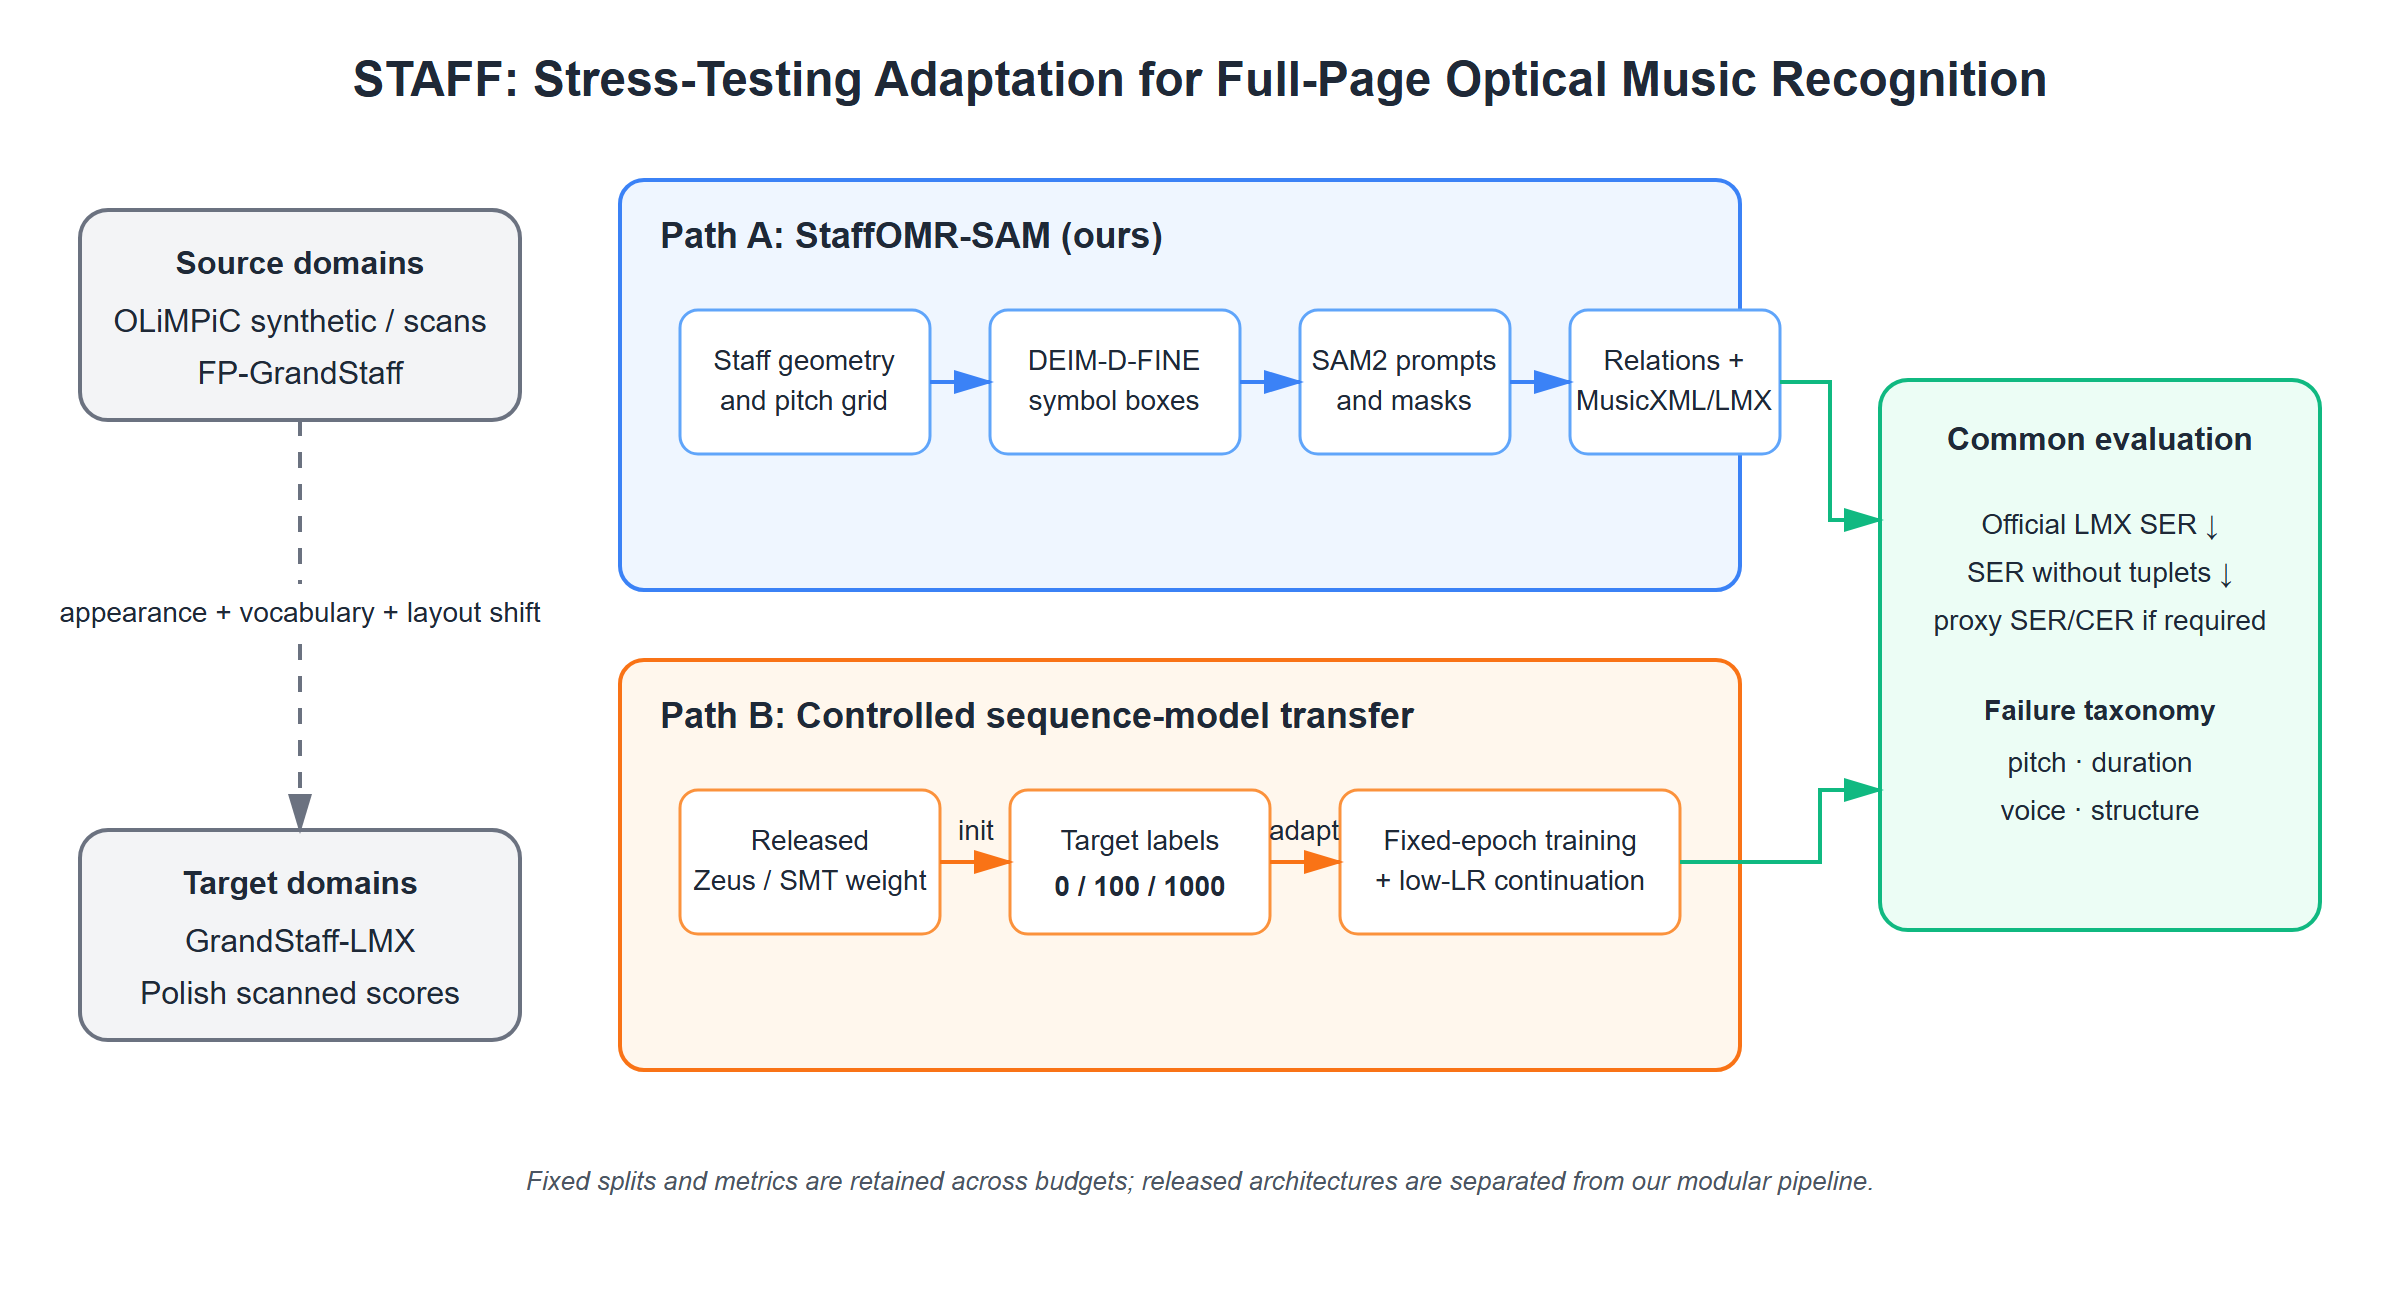
\includegraphics[width=0.96\textwidth]{staff_overview.png}
  \caption{STAFF keeps a modular, inspectable OMR path separate from controlled adaptation of released sequence models. Both paths feed a common evaluation and failure taxonomy.}
  \label{fig:overview}
\end{figure*}

\subsection{Path A: StaffOMR-SAM}
The modular path begins with horizontal projections and connected components to estimate five-line staff groups. For staff $k$, the detected line coordinates $\{\ell_{k,j}\}_{j=1}^{5}$ define a robust staff spacing $s_k$ and a half-space pitch grid. All subsequent windows, distance thresholds, and relation tolerances are normalized by $s_k$, making the geometric prior resolution-aware.

A DEIM-D-FINE detector predicts class-labeled boxes. DEIM supplies denser matching supervision, while D-FINE refines box-location distributions \cite{huang2025deim,peng2025dfine}. Full-page and staff-crop predictions are fused using class-aware non-maximum suppression. A lightweight crop classifier is used only within compatible symbol families; for example, the four-class clef classifier is not permitted to relabel noteheads or rests.

Each box becomes a prompt for SAM2. Prompt expansion and negative points depend on the symbol class: noteheads permit internal overlap with staff lines; stems suppress long horizontal components; beams retain thick elongated regions; ledger lines must remain short and close to noteheads. The resulting mask is converted to a polygon for area-like symbols or a pruned skeleton for stems, beams, ledger lines, barlines, and slurs. This design uses promptable segmentation as a boundary proposal mechanism rather than a notation recognizer.

Finally, normalized geometric rules assemble a relation graph. Candidate edges include notehead--stem, stem--beam, ledger--notehead, accidental--note, and slur-endpoint relations. Graph nodes are mapped to note/rest events, approximate pitch, measure position, and draft MusicXML/LMX. Figure~\ref{fig:overlay} shows that the pipeline exposes staff grids, boxes, and relations even when the semantic output remains incorrect.

\begin{figure}[t]
  \centering
  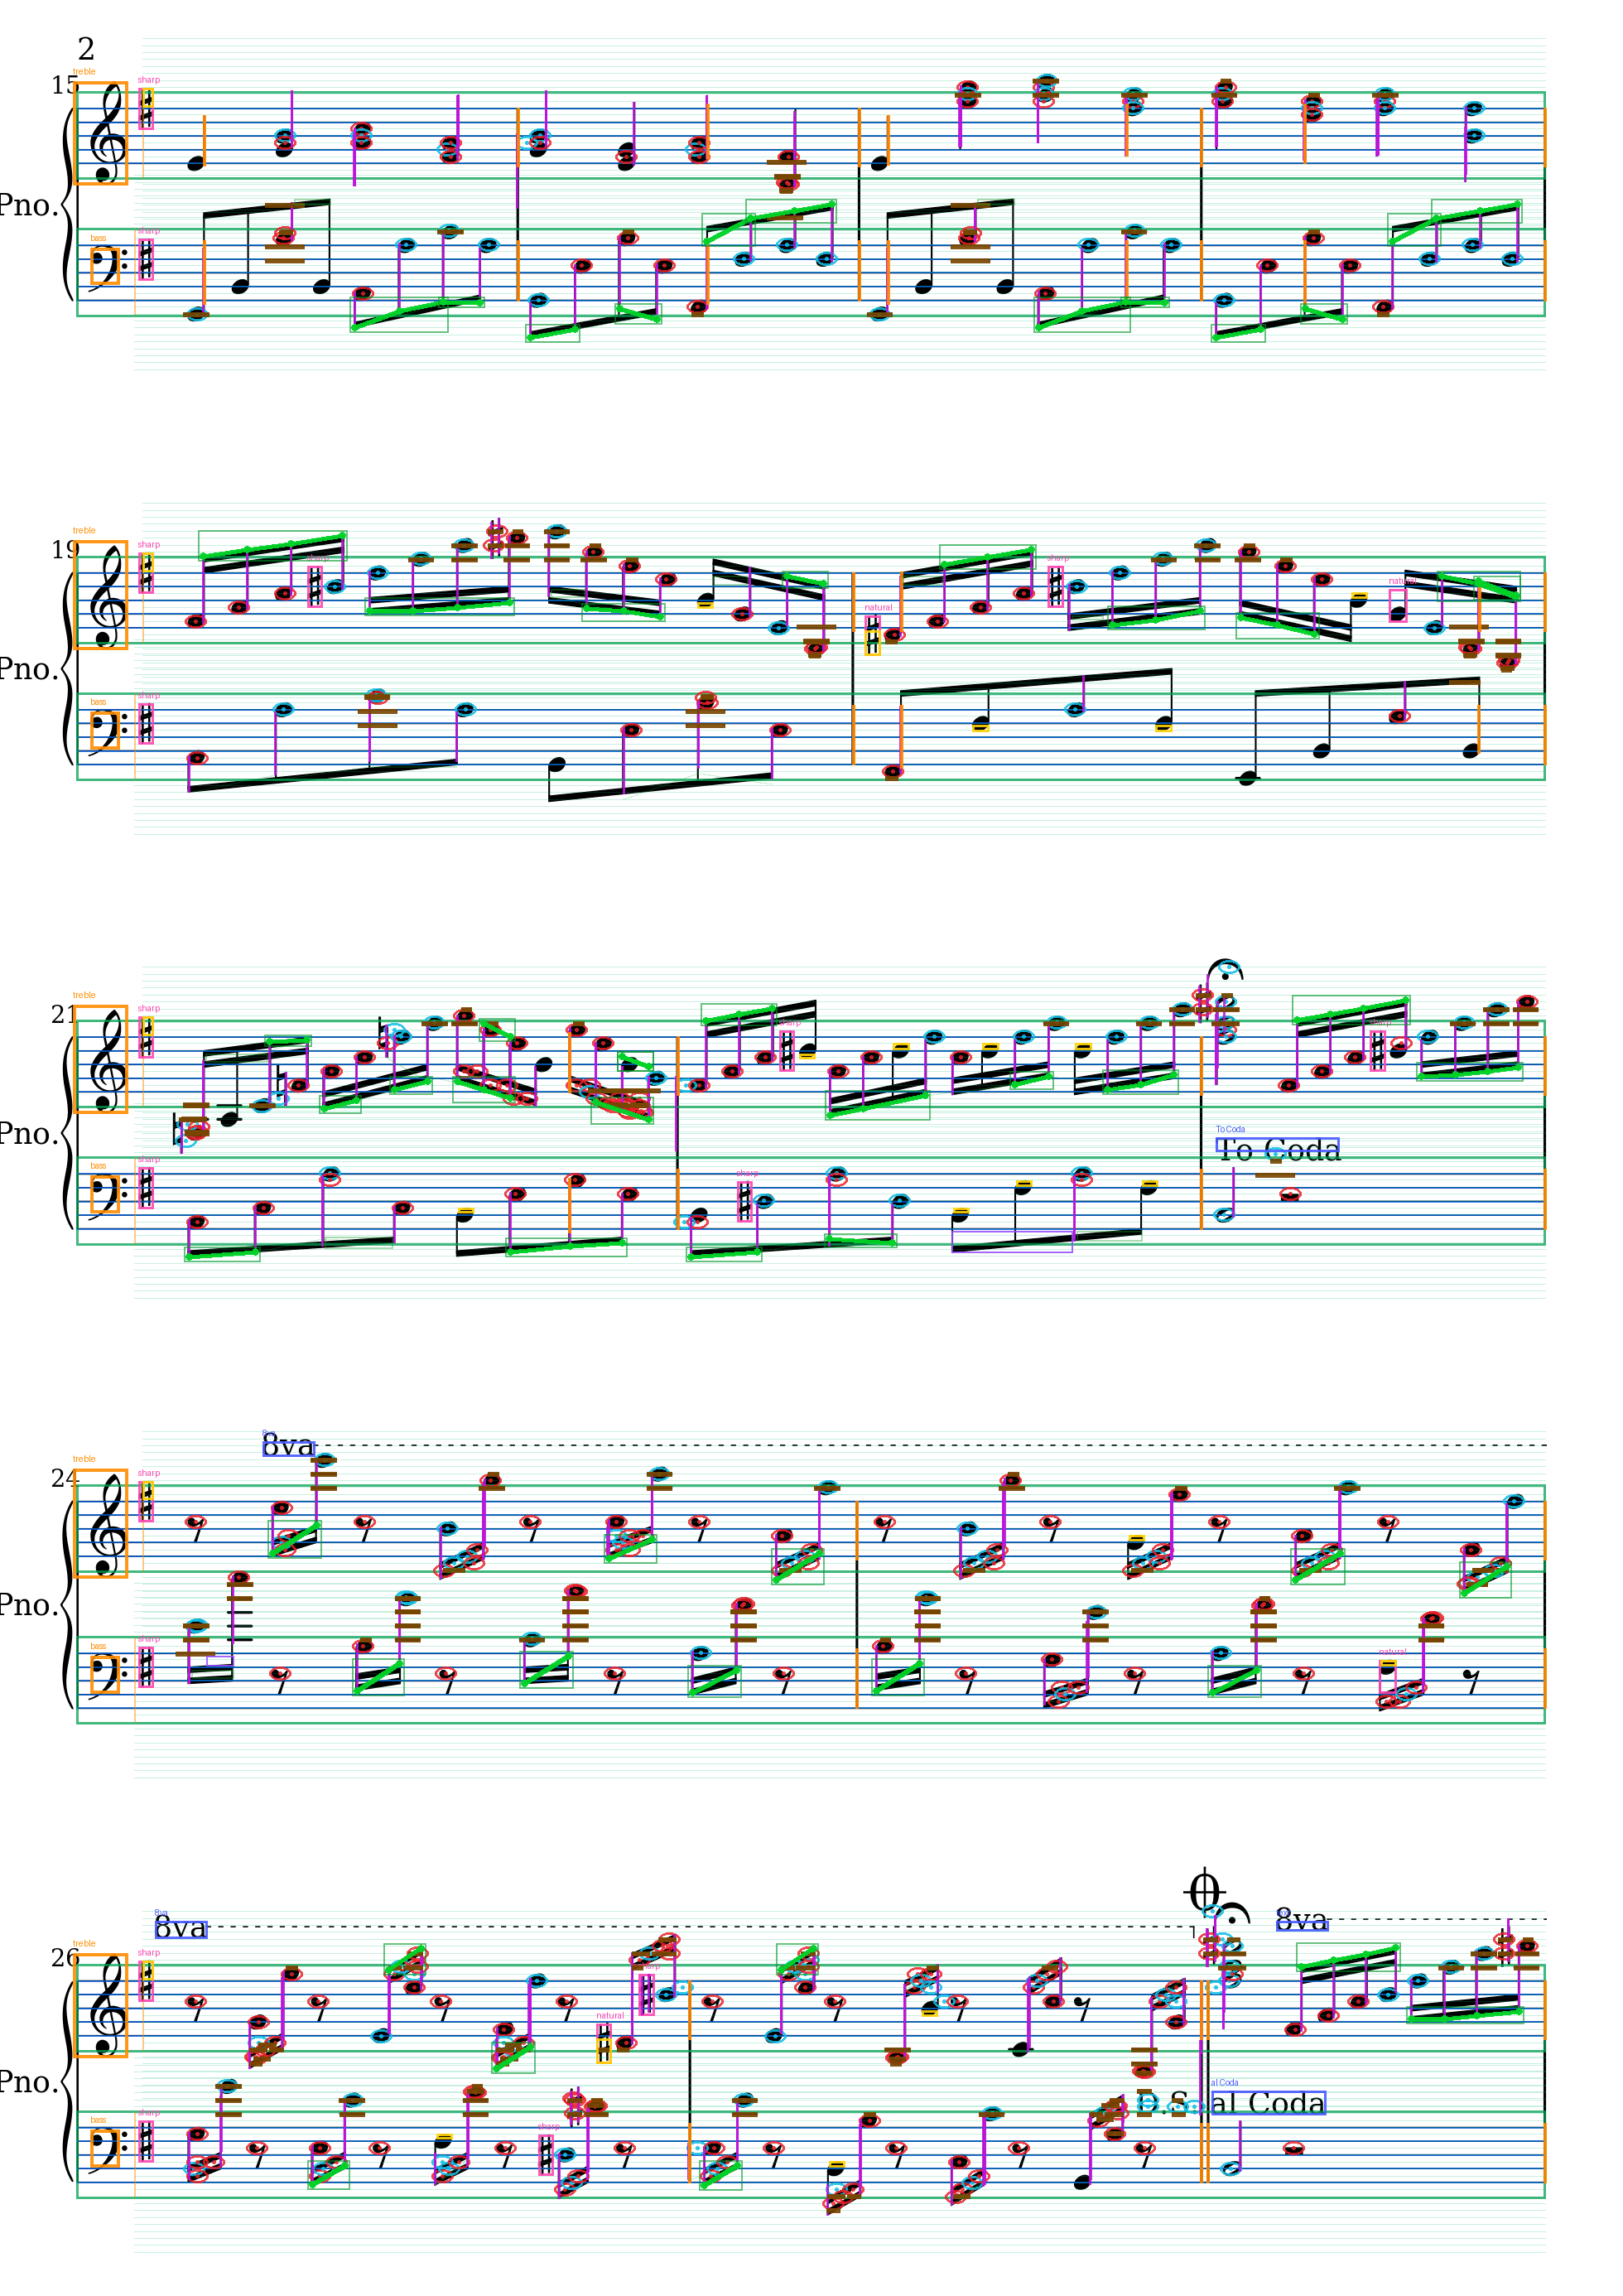
\includegraphics[width=\linewidth]{staffomr_overlay.png}
  \caption{Inspectable StaffOMR-SAM output on a dense piano page. Colored staff grids, symbol boxes, stems, beams, accidentals, and text regions enable component-level error attribution.}
  \label{fig:overlay}
\end{figure}

\subsection{Path B: Controlled Sequence Adaptation}
The sequence path initializes from a released source checkpoint. Its visual encoder and autoregressive Transformer decoder follow the standard image-to-sequence factorization
\begin{equation}
 p(y\mid x)=\prod_{t=1}^{T}p(y_t\mid y_{<t},f_\theta(x)),
\end{equation}
where $f_\theta$ is the image encoder. We fine-tune on exactly $B$ target pages, retain the released vocabulary unless an expanded-vocabulary run is explicitly identified, and use fixed-epoch training followed by a short lower-learning-rate continuation. AdamW is used for optimization \cite{loshchilov2019decoupled}. Model selection uses the designated development signal or the fixed checkpoint schedule recorded by the experiment; test-specific symbolic postprocessing is excluded from the headline test200 result.

For the main OLiMPiC-to-GrandStaff runs, training uses batch size 8, four data-loader threads, a learning rate of $10^{-4}$, and the released horizontal augmentation setting. The 100- and 1000-page subsets are disjoint from test200. Both use a fixed 20-epoch adaptation budget; the 100-page result additionally uses a recorded 10-epoch low-learning-rate continuation, while the 1000-page headline uses the best raw continuation checkpoint evaluated on the full 200-page test split. Runs were executed on CPU in the current reproduction environment. We report this detail because training hardware does not change the metric, but it affects reproducibility, wall-clock planning, and the temptation to shorten a small-data run unequally.

The adapted decoder is not given StaffOMR-SAM boxes, masks, or graphs. Likewise, the modular pipeline is not allowed to import the target sequence model's predictions. Keeping the two paths independent is intentional: a failure shared by both paths is more likely to be a protocol or representation problem, whereas a failure unique to one path localizes the modeling bottleneck. Hybrid fusion is deferred until each path has a stable, separately auditable baseline.

\section{Experiments}
\subsection{Datasets and Settings}
OLiMPiC provides pianoform systems with LMX targets and scanned evaluation material \cite{mayer2024practical}. GrandStaff-LMX is derived from the GrandStaff pianoform setting with an LMX-compatible evaluation view \cite{riosvila2023grandstaff}. FP-GrandStaff contains synthetic full pages, while the Polish collection contains 117 real scanned piano pages in the full-page study; our public local split contains 83 training and 24 test pages \cite{riosvila2026fullpage}. Because the Polish training split has only 83 pages, we report its full available budget rather than duplicating samples to fabricate 100 or 1000-page conditions.

The main transfer direction initializes the released OLiMPiC sequence checkpoint and adapts it to GrandStaff-LMX. The reverse direction initializes the released GrandStaff checkpoint and adapts it to OLiMPiC. The modular StaffOMR-SAM path uses no target-domain sequence training. We also report the released in-domain checkpoints as reference points, not as our results.

\subsection{Reproducibility and Selection Discipline}
Every evaluated item writes the predicted sequence, the reference sequence identifier, per-item edit counts, and a corpus summary. The modular path additionally writes detector predictions, staff geometry, masks or shape descriptors, relation edges, draft MusicXML, and visual overlays. Failed MusicXML construction is recorded explicitly. This artifact trail allows a corpus score to be traced back to a missing staff marker, illegal chord, empty prediction, or local symbol error.

Hyperparameter sweeps are separated from headline claims. StaffOMR-SAM geometric thresholds are calibrated on designated local material and then fixed for the cross-domain run. Sequence checkpoints are selected by the recorded schedule; we do not search the 200-page test split for a symbolic rewrite. This distinction matters because a rule that helps a 20-page diagnostic subset can harm the larger split, as shown by the tuplet ablation below.

\subsection{Main Results}
Table~\ref{tab:main} reports the central budget curve. Zero-shot transfer from OLiMPiC to GrandStaff-LMX produces 53.19\% SER on test200. One hundred target pages reduce SER to 38.18\%, and 1000 pages reduce it to 14.01\%. The in-domain GrandStaff checkpoint reaches 1.44\%, showing that a substantial gap remains even after 1000-page adaptation. Training the same small sequence architecture from scratch on 100 or 1000 pages was unstable in our local ablation and exceeded 200\% SER on test20, indicating that the gain comes from pretrained sequence knowledge rather than the target subset alone.

\begin{table}[t]
\caption{GrandStaff-LMX transfer results. Lower is better. ``No tup.'' ignores tuplet tokens. The in-domain row is a released reference checkpoint.}
\label{tab:main}
\centering
\small
\begin{tabular}{lrrr}
\toprule
Initialization / adaptation & Pages & SER & No tup. \\
\midrule
Released OLiMPiC, zero-shot & 0 & 53.19 & 52.87 \\
Adapted released model & 100 & 38.18 & 35.48 \\
Adapted released model & 1000 & \textbf{14.01} & \textbf{14.25} \\
Released GrandStaff, in-domain & full & 1.44 & 1.49 \\
\bottomrule
\end{tabular}
\end{table}

The reverse direction is less data-efficient (Table~\ref{tab:reverse}). The released GrandStaff checkpoint obtains 56.49\% SER on OLiMPiC test200; adaptation with 100 target pages lowers SER to 51.79\%. The modest improvement contrasts with the 15.01-point reduction in the 100-page GrandStaff direction. This asymmetry is consistent with simultaneous appearance and vocabulary shift: a target subset may teach common tokens without covering rare constructs or scanned-image variation.

\begin{table}[t]
\caption{Reverse transfer to OLiMPiC test200.}
\label{tab:reverse}
\centering
\small
\begin{tabular}{lrrr}
\toprule
Initialization / adaptation & Pages & SER & No tup. \\
\midrule
Released GrandStaff, zero-shot & 0 & 56.49 & 50.63 \\
Adapted released model & 100 & \textbf{51.79} & \textbf{47.80} \\
Released OLiMPiC, in-domain & full & 13.29 & 9.53 \\
StaffOMR-SAM + crop fusion & 0 & 74.42 & 73.57 \\
\bottomrule
\end{tabular}
\end{table}

\subsection{Ablations and Negative Results}
Table~\ref{tab:ablation} records interventions that would be easy to omit from a success-only narrative. On GrandStaff-LMX test20, repairing illegal chord structure removes five construction failures and improves SER by 4.80 points. Official-style export and threshold calibration improve it further, but the final 76.31\% remains weak. Dropping predicted tuplets from the adapted sequence output appears helpful on test20, reducing 33.20\% to 29.94\%, yet it degrades test200 from 14.01\% to 21.17\%. The correct interpretation is not that tuplets should be suppressed, but that a small diagnostic split supported a non-general rule.

\begin{table}[t]
\caption{Selected ablations. Lower SER is better. Results on different test sizes are not directly pooled.}
\label{tab:ablation}
\centering
\small
\begin{tabular}{llrr}
\toprule
Path & Variant & $N$ & SER \\
\midrule
Modular & raw MusicXML & 20 & 86.48 \\
Modular & + chord legality & 20 & 81.68 \\
Modular & + official-style export & 20 & 76.31 \\
Sequence & adapted raw checkpoint & 20 & 33.20 \\
Sequence & + drop tuplets & 20 & \textbf{29.94} \\
Sequence & adapted raw checkpoint & 200 & \textbf{14.01} \\
Sequence & + drop tuplets & 200 & 21.17 \\
\bottomrule
\end{tabular}
\end{table}

Training from scratch supplies another negative result. A locally instantiated small sequence model trained on 100 GrandStaff pages obtains 262.52\% SER on test20; increasing the subset to 1000 pages still yields 249.08\%. Error rates can exceed 100\% because insertion counts are unbounded relative to the reference length. These runs do not prove that training from scratch is impossible, but they show that the present budget and schedule are insufficient and that the successful adaptation curve depends on source pretraining.

\subsection{Modular Path and Auxiliary Classifier}
StaffOMR-SAM completes all 200 OLiMPiC examples, but its 74.42\% SER is not competitive with either released sequence checkpoint. On GrandStaff-LMX test20, raw MusicXML produces five invalid-structure failures and 86.48\% SER. A chord-legality repair removes the failures and reduces SER to 81.68\%; an official-style export and threshold sweep reach 76.31\%. These gains confirm that structural validity matters, but their scale is too small to explain the full performance gap.

The family-constrained crop classifier offers a cleaner component-level result. A four-class clef model trained on 5,629 crops and evaluated on 1,422 validation crops reaches 98.10\% accuracy. Treble and bass clefs each reach 100\%, alto C clef reaches 97.65\%, and tenor C clef reaches 87.43\%. Yet adding scan-augmented crop fusion changes OLiMPiC SER only from 74.54\% to 74.42\%. Strong local classification therefore does not imply strong semantic transcription.

\subsection{Transfer Beyond the LMX Protocol}
The Polish and FP-GrandStaff experiments use a separate eKern-compatible proxy and are therefore summarized in Table~\ref{tab:proxy}, outside the LMX tables. The results reinforce two observations without supporting a cross-metric ranking. First, the released FP-GrandStaff SMT checkpoint transfers very poorly to Polish scans: proxy SER is 153.00\% and proxy CER is 141.76\%. Fine-tuning on all 83 available Polish training pages reduces these errors to 107.97\% and 125.30\%, respectively, but remains weak in absolute terms. Second, the modular StaffOMR-SAM pipeline obtains 98.86\% proxy SER without Polish sequence training. This is lower than the adapted SMT value under the local proxy, but it does not establish superiority under official LMX or a full-page structural metric.

\begin{table}[t]
\caption{Cross-domain eKern proxy results. These values are not comparable to official LMX SER. Lower is better.}
\label{tab:proxy}
\centering
\small
\begin{tabular}{llrr}
\toprule
Target & Method / budget & SER & CER \\
\midrule
Polish & StaffOMR-SAM / 0 & 98.86 & \textbf{64.02} \\
Polish & + crop fusion / 0 & \textbf{98.73} & 64.13 \\
Polish & released SMT / 0 & 153.00 & 141.76 \\
Polish & adapted SMT / 83 & 107.97 & 125.30 \\
FP-GS & StaffOMR-SAM / 0 & 109.17 & 67.17 \\
FP-GS & + crop fusion / 0 & \textbf{102.69} & \textbf{62.39} \\
\bottomrule
\end{tabular}
\end{table}

Crop fusion has dataset-dependent effects. On FP-GrandStaff it improves proxy SER by 6.48 points and CER by 4.78 points, suggesting that synthetic full pages contain symbol-family confusions that the constrained classifier can repair. On Polish, it improves SER by only 0.13 point and worsens CER by 0.11 point. The same component therefore helps on clean rendered pages but is neutral on historical scans. This difference is consistent with the appearance gap in Figure~\ref{fig:domain}: local crop classification cannot repair missed systems, degraded marks, or global reading order.

These proxy experiments also illustrate why metric provenance must be part of a transfer claim. Two evaluators may both report ``SER'' while tokenizing chords, voices, tuplets, or line structure differently. STAFF records the evaluator and encoding next to every result, and a future unified release should translate all predictions into LMX or MusicXML before aggregating domains.

\section{Analysis}
\subsection{Where Transfer Fails}
We align predicted and reference tokens and group errors into four categories. \emph{Pitch} errors arise from clef, accidental, octave, and staff-relative location mistakes. \emph{Duration} errors include note value, beam/flag interpretation, dots, and tuplets. \emph{Voice} errors cover chord grouping, staff assignment, backup operations, and reading order. \emph{Structure} errors include missing measures, invalid MusicXML events, and vocabulary mismatch.

\begin{table*}[t]
\caption{Failure taxonomy used to connect sequence errors to actionable model changes.}
\label{tab:errors}
\centering
\small
\begin{tabular}{lp{0.34\textwidth}p{0.38\textwidth}}
\toprule
Category & Observable symptom & Likely intervention \\
\midrule
Pitch & wrong clef, step, octave & staff-conditioned decoding \\
Duration & flag, dot, tuplet error & attachment-aware rhythm model \\
Voice & missing backup/chord order & constrained voice state \\
Structure & invalid or missing measure & grammar-valid decoder \\
\bottomrule
\end{tabular}
\end{table*}

This taxonomy is deliberately output-oriented. Detector average precision alone cannot tell whether two correctly localized noteheads were assigned to the wrong voice, whether a beam changed duration, or whether a syntactically valid token sequence represents an impossible measure. Conversely, sequence SER alone does not reveal whether a pitch error originated in staff localization, clef recognition, or decoding. The paired artifact trail connects these levels without pretending that one metric subsumes the other.

The modular pipeline is strongest at making the first two visual stages inspectable but weakest at converting local detections into globally valid voice and measure structure. Conversely, an autoregressive decoder can learn structural regularities but degrades when the page style and vocabulary move outside its training distribution. The paired results suggest that a future hybrid should not merely concatenate detector features with a decoder. It should expose staff, measure, and attachment constraints during decoding and retain a common LMX evaluation.

\subsection{Toward a Structure-Constrained Hybrid}
The evidence suggests three concrete next steps. First, staff and measure coordinates can be encoded as explicit positional channels or discrete tokens so that the decoder does not need to relearn page geometry after every engraving shift. Second, attachment candidates from polygons and skeleton endpoints can restrict which noteheads, stems, beams, and accidentals may form an event. Third, a grammar state can prevent illegal MusicXML operations during beam search. Each intervention corresponds to one row of Table~\ref{tab:errors} and can therefore be evaluated with both category-level errors and corpus SER.

Such a hybrid must still preserve the label-budget protocol. Adding structure is useful only if it improves zero-shot transfer or reduces the number of target pages needed to reach a fixed SER. A larger in-domain model that consumes more labeled target data would not answer the same question. The principal experimental target for the next version is therefore the area under the transfer curve over $B\in\{0,100,1000\}$, accompanied by in-domain accuracy and category-level failure counts.

\subsection{What the Label-Budget Curve Reveals}
The 100-page result is important precisely because it is not near the in-domain ceiling. It recovers 15.01 SER points, whereas the next 900 pages recover another 24.17 points. Reporting only the 1000-page result would hide the poor ultra-low-data regime; reporting only zero-shot transfer would understate the value of adaptation. A budget curve also prevents incomparable claims in which one method receives scanned target pages and another does not.

Tuplet suppression illustrates a second protocol risk. On GrandStaff-LMX test20, a test-specific postprocess lowers full SER from 33.20\% to 29.94\%, but applying the same rule to test200 worsens full SER from 14.01\% to 21.17\%. We therefore report the raw test200 checkpoint as the main result. Small development sets can make symbolic rules look universally beneficial when they are not.

\section{Limitations and Responsible Use}
STAFF is an empirical first version. The available target budgets are not yet complete in both directions, the Polish evaluation uses a proxy token protocol rather than official LMX, and the modular pipeline remains far from competitive semantic accuracy. The current evidence does not establish a new OMR state of the art or a general domain-adaptation algorithm. It establishes a reproducible diagnosis and identifies where additional modeling is required.

The datasets contain public-domain or research-licensed score images, but future deployment on contemporary editions must respect copyright and dataset licenses. OMR output can also be used in educational feedback; inaccurate pitch or rhythm transcriptions must not be presented to students as authoritative. A practical system should expose confidence, preserve the source image, and support human correction rather than silently generating a definitive score.

\section{Conclusion}
STAFF evaluates OMR as a cross-domain transfer problem rather than a single in-domain benchmark. Controlled adaptation of a released OLiMPiC model reduces GrandStaff-LMX test200 SER from 53.19\% to 38.18\% with 100 target pages and 14.01\% with 1000 pages, while reverse transfer remains much harder. A complementary staff-aware detector--segmenter--graph pipeline exposes useful intermediate geometry but confirms that local recognition is not enough: voice, duration, pitch, and global structure dominate the remaining semantic error. The immediate research direction is therefore constrained sequence adaptation informed by explicit staff and relation structure, evaluated under fixed label budgets and official metrics.

\bibliography{staff_refs}
\end{document}
